\subsection{UC27 - Visualizzazione errore dimensioni bin non valide}
\begin{figure}[H]
  \centering
  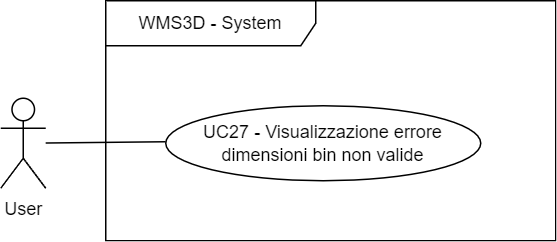
\includegraphics[width=0.8\textwidth]{UC_diagrams_21-27/UC27.drawio.png}
  \caption{Diagramma UML UC26 - Visualizzazione errore posizione non valida}
\end{figure}
\begin{itemize}
    \item \textbf{Attori:} User.
    \item \textbf{Pre-condizione:}  L'utente sceglie una dimensione per il bin della scaffalatura che eccede i confini del magazzino o che è più piccola delle dimensioni minime previste.
    \item \textbf{Post-condizione:} L'utente visualizza un messaggio d'errore e le dimensioni del bin non vengono inserite.
    \item \textbf{Scenario Principale:} L'utente visualizza un messaggio informativo sull'errore.
    \item \textbf{Generalizzazioni:} -
    \item \textbf{Estensioni:} -
\end{itemize}